\documentclass[a4paper,12pt]{article}
\usepackage[utf8]{inputenc}
\usepackage{tabularx}
\usepackage{amssymb}
\usepackage{hhline}
\usepackage{graphicx}
\usepackage{pstricks-add}
\newcommand{\intinf}{\int_{-\infty}^{\infty}}
\newcommand{\sumg}{\sum_{\gamma=0}^{2k}}
\newcommand{\spl}{\psi^{(k+1)}}
\usepackage{pgf,tikz}
%\usepackage[toc,page]{appendix}
%
% \usetikzlibrary{arrows}
\usepackage{rotating}
\usepackage{lscape}
\usepackage{epstopdf}
\newtheorem{theorem}{Theorem}[section]
\newtheorem{definition}{Definition}[section]
\usepackage{enumerate}% http://ctan.org/pkg/enumerate
\usepackage{pgf,tikz}
\usepackage{caption}
\usepackage{subcaption}
\usepackage{pdflscape}
\bibliographystyle{plain} % or: "chicago"
\usepackage[utf8]{inputenc}
\usepackage{amsmath}
\usepackage{amsfonts}
\newtheorem{note}{Note}[section]
\usepackage{amssymb}
\usepackage{graphicx}
\usepackage{pstricks-add}
\usepackage{float}    
%\usepackage{multirow}
\newtheorem{proposition}{Proposition}
\newtheorem{lemma}{Lemma}
\setcounter{section}{0}
\usepackage{listings}
\author{Julia Docampo}
\newcommand{\xin}{x_{i-\frac 12}}
\newcommand{\xip}{x_{i+\frac 12}}
\usepackage{pgf,tikz}
\usetikzlibrary{arrows}
\usetikzlibrary{decorations.markings}
\usepackage{rotating}
\usepackage{lscape}
\usepackage{epstopdf}
\newtheorem{lema}{Lemma}[section]
\newtheorem{remark}{Remark}[section]
\newtheorem{corollary}{Corollary}[section]
%\usepackage{subfig}
%\newtheorem{proposition}{Proposition}[section]
\usepackage{enumerate}% http://ctan.org/pkg/enumerate
\newcommand*{\QEDA}{\hfill\ensuremath{\blacksquare}}%
\newcommand*{\QEDB}{\hfill\ensuremath{\square}}%
\usepackage{pgf,tikz}
\usetikzlibrary{positioning,arrows}
\usepackage{natbib}
\usepackage{etex}

\usepackage{color}
 
 \begin{document}
 
 
 %section{Introduction}
 \section{Introduction}
 
 Curve and surface modeling play a major role in Reverse Engineering during object reconstruction
  through CAD software \cite{Ma1998, sarkar1991} as well as for CFD simulations involving moving
  interfaces such as flame propagation problems \cite{malladi1995}. 
  The typical situation is that one has access only to a discrete (finite) data set 
  and a smooth curve (surface) is needed in order to perform operations such as numerical integration or differentiation. 
  Although not unique, the solution to this problem is generally sought as a spline curve (surface)  
  that either interpolates the data or provides an approximation which is \emph{closest} to it.
   An approximation \emph{fit} is more desirable for experimental measurements or computational data 
   which may be slightly inaccurate or noisy whereas an interpolating approach \cite{piegl1999,ma1995} 
   is more suitable when
   the data (or part of it) is known to be exact. This paper focuses on 
   approximation techniques since the algorithm presented here was developed for 
    curve reconstruction for numerical solutions on aircraft icing accretion \cite{}. 
    
    Splines are determined by the approximation degree, 
    control polygon (net) and knot sequence. The ideal spline \emph{fit} is an approximation
     that minimizes the error (under certain metric) employing a minimum number 
     of knots (control points).  Unfortunately, this represents a great challenge since both the ``optimal'' number of control points 
  and knot location are unknown and in general, it is not possible to derive explicit formulas \cite{jupp1978}.  
  Thus, the solution is found by casting a suitable optimization problem, 
  usually based on the least-squares minimization \cite{nurbs_book, deboor2001practical, schumaker2015spline}. 
   The methodology proposed here attempts to solve the \emph{minimal} spline problem 
    heuristically by inserting knots 
   as part of an iterative scheme that drives the solution towards a desired accuracy. 
      
  The simplest solution to the spline least-squares optimization problem is to fix the 
  knot sequence (number and distribution) alongside a suitable curve parametrization and solve a linear system for the 
  control points \cite[Ch. 9.4]{nurbs_book}, \cite{deboor1968}. 
  The usual parametrization choices are based on the chord-length or centripetal models  which 
  have proven to improve the quality of the approximation, 
  especially for detection of sharp features such as ``cusps'' \cite{hoschek1988,speer1998,lee1989, ma1995}. 
  However,  a fixed knot sequence may be too oversimplified and 
  shape manipulation (knot insertion/removal) \cite{piegl1989, boehm1980, goldman1992} 
   can be introduced as part of an error controlled iterative scheme. For example, 
    continuously inserting knots and applying least-squares minimization 
   ($i.e.$ finding new control points) until a specified tolerance is attained
    \cite{piegl2000, park2007}. Alternatively, one can starting with a large number 
    of control points and remove knots successively as long as the 
     quality of the approximation is not destroyed \cite{lyche1987, tiller1992}. 
   Ultimately, the problem can be formulated as a non-linear optimization, allowing 
   ``free knots'' as part of the least-squares solution \cite{schwetlick1995least, beliakov2004}. 
   The free-knots problem generally yields to better results but this occurs at the expense 
   of computational efficiency \cite{randrzanarivony2002}. In addition, it can result 
   in many stationary points \cite{jupp1978}.
   
   This paper presents a new algorithm from the \emph{knot insertion} category; 
   starting with a minimum number of knots, we look for the span with greatest weighted error, 
   insert a new knot and find the control points using a linear least-squares solver. 
   If the new approximation is above the tolerance step, the knot sequence is updated. 
   Otherwise, the step is rejected and a new knot is inserted at the next  "high-error" span. 
   When no new knots overcome the step control, the scheme proceeds with the "best so far", 
   tags the knot location and when a valid step is found, 
   attempts to remove any potential redundant knot. 
    The algorithm stops if either the global error hits the desired tolerance (1), it has 
    reached the maximum number of iterations (2) or no new knots can 
    improve the current approximation (3). 
  Although we cannot prove that this strategy is optimal,
  our results suggest that this knot distribution leads to accurate results
  remaining at relatively low computational costs, thus becoming suitable  for engineering applications. 
  
   
   In the following sections we discuss the different aspects of our method. Section \ref{} defines 
   the algorithm building blocks: Bspline functions, 
   least squares approximation and the ``best knot'' sequence problem. 
   In section \ref{} implementation details are given and section 
   \ref{} shows the results of applying this tool on several data  types 
   including curve fitting on noisy noisy data as well as ice-layer reconstruction. 
   Finally,  in section \ref{}  we conclude and highlight the areas for improvement as well as future applications.
 
 
 
   \section{Background}
  
%  In the following, we will discuss the building blocks of our algorithm, namely 
%   B-spline functions, least-squares curve fitting and the knot sequence problem. Then we provide a full description of our 
%   algorithm 
We begin by introducing B-spline functions together with formulas for their computation and 
describe the components of a B-spline curve. 
We assume that the reader is familiar with these functions and full details can be found in 
 \cite{nurbs_book, deboor2001practical, schumaker2015spline}. 
  \subsection*{B-splines and Least Squares Approximations}
% Here we provide formulas for computing B-splines together with a brief discussion of its components  
% and for full details, we refer the reader to .
B-spline curves are fully determined by the approximation degree, 
knot sequence and control polygon. Given a knot sequence $U=\left\{u_0,\ldots,u_r\right\}$ satisfying 
 $u_i\leq u_{i+1},\  i=0,\ldots r-1$, we define 
 the $i^{th}$ B-spline of degree $p$ through the recurrence formula:
 \begin{align}
 N_{i,0} &= \left\{ \begin{aligned}
                    1 \quad &\text{if } u_i\leq t\leq u_{i+1}\\
                    0 \quad &\text{otherwise }
                   \end{aligned}\right. \\
N_{i,p} &= \frac{t - u_i}{u_{i+p} - u_i}N_{i,p-1}(t) +  \frac{u_{i+p+1} - t}{u_{i+p+1} - u_{i+1}}N_{i+1,p-1}(t).
 \end{align}
 Given a data set $\left\{X_i\right\}_{i=1}^m$, and a fixed knot sequence $U=\{u_0,\ldots,u_r\}$, 
 we 
look for the B-spline curve 
\begin{equation}
 C(t) = \sum_{i=0}^{n=r-p-1} N_{i,p}(t)\cdot \mathbf P_i,\quad \mathbf P_i = \text{control point} ,\quad t\in[0,1]
\end{equation}
that approximates the data in the least squares sense:
\begin{align}\label{eq:least_squares_problem}
 & C(0)= X_0, \quad \  C(1) = X_m\quad \text{and}\\
 &\sum _{k= 1}^{m-1}\left | X_k - C(t_k)\right|^2\quad \text{is a minimum with respect }\mathbf P_i.
\end{align}
Figure \ref{fig:bspline_sine} shows an example of a B-spline curve approximating a planar sine-wave.
The pairs $(t_k,X_k)$ are associated through a well-suited parametrization 
which in our case corresponds to the centripetal method \cite{lee1989}:
\begin{align}
 t_0 &= 0,\quad t_m = 1\\
 t_k &= t_{k-1} + \frac{\sqrt{ |X_k - X_{k-1}|}}{\sum_{i = 1} ^ m \sqrt{|X_i- X_{i-1}|}}, \quad k = 1,\ldots,m-1.
\end{align}
The centripetal model intends to capture sharp features on the data but alternatively, 
one can use an uniform \cite{} parametrization, chord-length \cite{} 
and more recently \cite{}. 

\begin{figure}
 \centering
 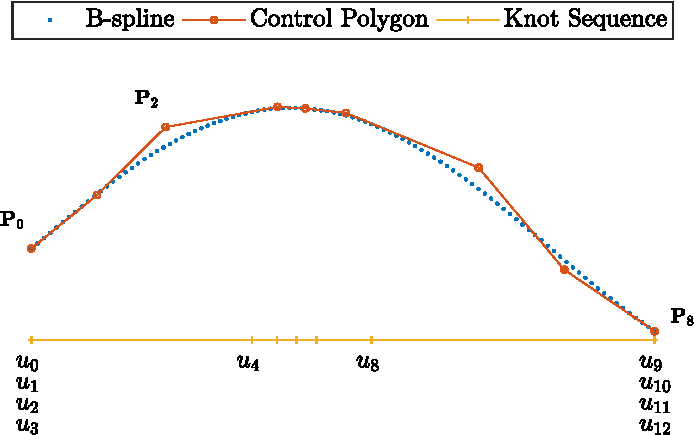
\includegraphics[width =0.75\textwidth]{sinePlot/sineBspline-crop}
 \caption{\label{fig:bspline_sine} A cubic B-spline curve approximation to a piece of a sine wave employing nine
 control points ant the knot sequence 
 $U=\left\{u_0,\dots,u_{12}\right\}$.}
\end{figure}
 

The solution to equation \eqref{eq:least_squares_problem} can be found as follows \cite[Ch. 9.4.1]{nurbs_book}. 
Let  
\begin{equation}
 R_k = Q_k - N_{0,p}(t_k)\cdot Q_0 - N_{m,p}(t_k)\cdot Q_m,  \quad k = 1,\ldots, m-1.
\end{equation}
Since the B-spline knots are fixed, minimizing for the control points gives:
\begin{equation}\label{eq:linear_least_squares_solver}
 \sum_{i=1}^{n-1} \left( \sum_{k=1}^{m-1} N_{\ell, p}(t_k)\cdot N_{i,p}(t_k)\right)\cdot\mathbf P_i= \sum_{k=1}^{m-1}N_{\ell,p}(t_k)R_k, \quad \ell= 1\ldots, n-1
 \end{equation}
which we write in matrix notation as $(N^TN)\mathbf P = R$.
The Schoenberg
Schoenberg-Whitney condition \cite{} implies that 
\begin {equation}
 u_i < t_k < u_{i+k},\quad i = 1,\ldots,m ,
\end {equation}
then the matrix in \eqref{} has full rank and can be solved applying any linear matrix solver. Hence, each
 span must contain at least one $t_k$. 
\end{note}

The motivation for introducing iterative knot insertion is that equation \eqref{eq:least_squares_problem} 
requires \emph{a priori} knowledge on the amount of control points needed which is often unavailable. Furthermore, inserting new 
knots locally, at regions with high error, can  lead to a better approximation as shown in our results 
section ($e.g.$ Figure \ref{}). 
\subsubsection{Knot Placement}\label{sec:knot_placment}
Given an approximation degree ($p$), 
the knot insertion technique presented here starts with a minimum knot sequence
$U=\{0,\underbrace{\ldots}_{p-1},0,1,\underbrace{\ldots}_{p-1},1\}$.
%\begin{equation}\label{eq:clamped_knots}
%
%\end{equation}
Then, each iteration consists of finding the span with greatest weighted error: 
 $$e_k = \frac{1}{N_k}\sum_{i=1}^{N_k} (C(t_i) - X_i)^2,\quad N_k = \# t_i\in [u_k, u_{k+1}),\ i=1,\ldots,m-1, $$
 where the distance function is computed as follows:
 \begin{equation}\label{eq:distance_projection}
  C(t_i) - X_i = \min_{t\in[0,1]} |C(t) -  X_i|,
 \end{equation}
$i.e.$, the \emph{actual} distance to the data. The new knot position is determined by
 the first $t_i$ such that $t_i \geq \frac{e_k}{2}$ and takes
 the value $\tilde u = \frac{t_i+t_{i+1}}{2}$. 
 This knot choice ensures that the split $[u_i, \tilde u),\ [\tilde u,u_{i+1})$ are non empty spans 
 (see Note \ref{note:sw_cond}). 

 
 
 In \cite[Ch. ]{nurbs_book}, 
 it was propsed to find all the spans that are above a targeted tolerance and introduce a knot at the highest error. 
 However, this strategy does not account  
 for the fact that each knot has impact in more than one control point and it may lead to an excessive number
  of control points. It is well known that spline functions develop wiggles when employing a high number of control points; 
   if high error regions have few data support, iterative approximation may lead to ``jammed knots'' which might lead to local oscillations
   when each span is only supported by one data point. Such artifacts may not be visible to the Least-Squares solver 
   which is evaluating only at the parametrization values. This is shown in Figure \ref{fig:bspline_wiggle} where the resulting curve is shown at the values used during minimization (centripetal) 
and over an uniform sampling where we can see that wiggles have developped. This is because in that region, almost all the 
 knot spans contain only one $t-$value forcing the curve to interpolate through the data and producing a zig-zagging control polygon. 
   Finally, notice that for each data point $X_k$, 
   the error function from equation \eqref{eq:distance_projection} finds a parameter along the curve 
    taht doesn't necessarily coincide with $t_k$. Hence, when placing the knot at the maximum $t_k$, this doesn't reflect the actual position of this maximum. 
    Figure \ref{fig:knot_placement} shows an example of applying knot insertion based on half-way weighted error (see ), at the maximum error and at the middle of the span with 
    highest error. We can see that the weighted error produces the most accurate curve.  
 
 \begin{figure}
 \centering
  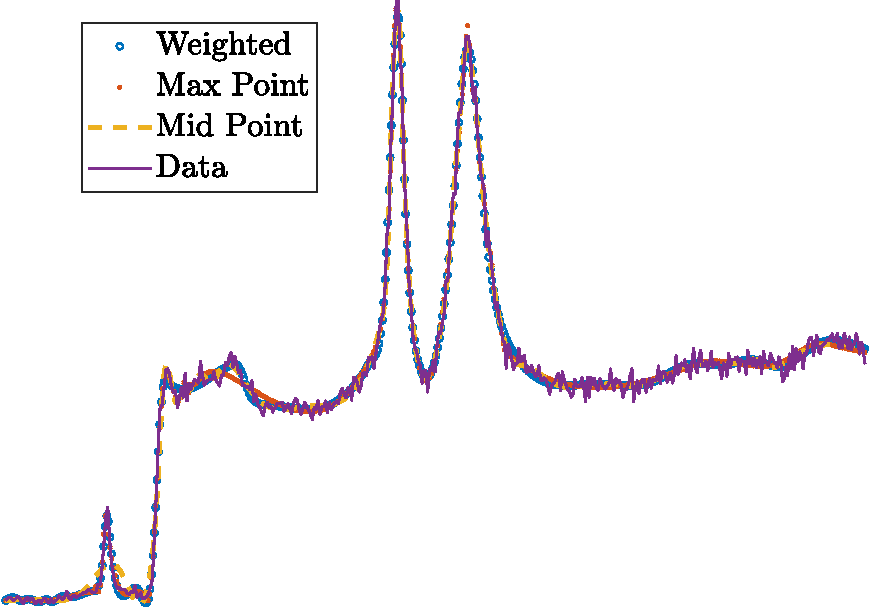
\includegraphics[width = \textwidth]{knot_placement_plot}
  \caption{\label{fig:knot_placement} Bspline curves employing a weighted error knot insertion, a maximum error position and at the middle of the span with greatest error. 
  The experimental data corresponds to a Ramana Spectroscopy.}
 \end{figure}

 
 \begin{figure}
  \centering
  \begin{tabular}{ccc}
  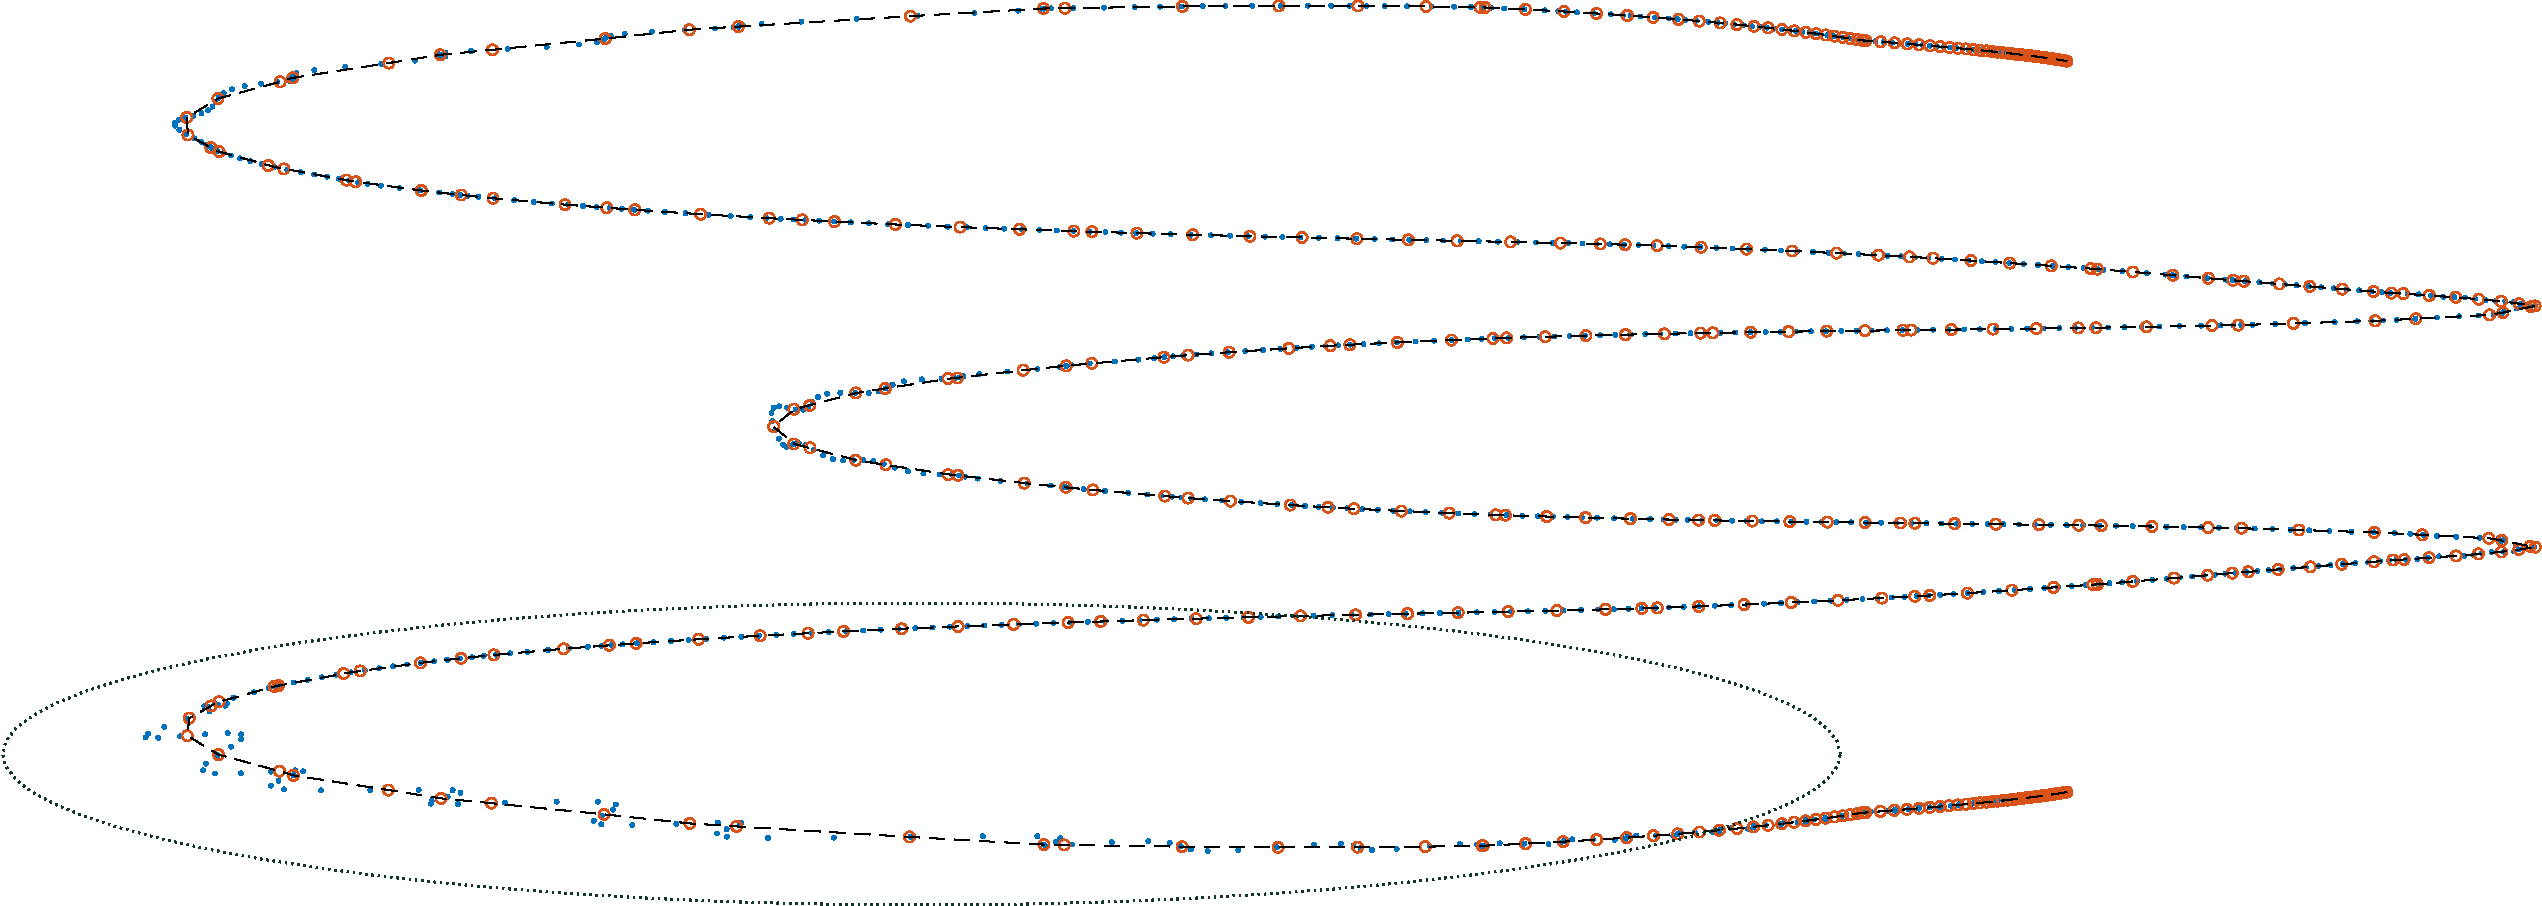
\includegraphics[width=0.45\textwidth,height= 0.3\textwidth]{ellipse-crop}&&
  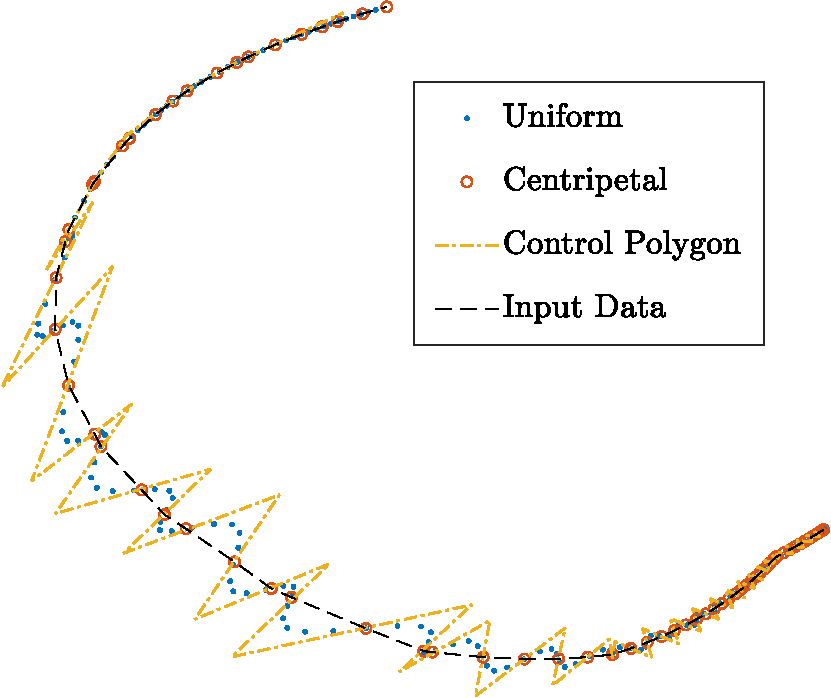
\includegraphics[width=0.45\textwidth,height= 0.3\textwidth]{wiggle_ALL-crop}
  \end{tabular}
\caption{\label{fig:bspline_wiggle}Curve reconstruction of a level set solution sampling the B-spline at 
the centripetal nodes and at a uniform sample. The rigth plot is a zoom of the highlighted region revealing the ``hidden'' wiggles.}
 \end{figure}


\subsubsection{The Algorithm}
Now that the least squares approach and knot placement have been discussed, we introduce the main algorithm and discuss implementation 
details. Once the desired tolerance is selected, we use the centripetal method in order to obtain a curve parametrization: 
\begin{align}
 d &= \sum_{k=1}^n \sqrt {| X_k-X_{k-1}|},\\
 t_0 &=0,\ t_m=1,\quad t_k = t_{k-1} + \frac{\sqrt{|X_k-X_{k-1}|}}{d},\quad k = 1,\ldots, m-1.
 \end{align}
This method has proven to be suitable for detecting curve features such as ``cusps'' \cite{}. 
\begin{note}
 If the initial number of control points is set $n > p$, we define the internal knots sequence proposed by proposed by \cite{}: 
  \begin{align}
  d &= \frac{m+1}{n-p+1} \Rightarrow i = int(j\cdot d),\quad \alpha = jd -i\\
  u_{p+j} &= (1-\alpha)u_{i-1} + \alpha u_i,\quad j = 1,\ldots,n-p.
 \end{align}
\end{note}

At each iteration, we solve \eqref{} and compute the global error. If we haven't reached the desired tolerance, 
we insert a knot as discussed in section \ref{sec:knot_placment} and find the new control points. If the 
new configuration has not significantly improved the previous iteration, we reject the knot and find the next worst error. 
 If all knots were found to be ``unsuitable'' we proceed with the best configuration, insert a new knot and tag its 
 value. Once a significant improvement has been found, we try to remove all the ``redundant'' points computed between the tagged knot and the 
 knot at valid iteration and when possible, the knots in between are removed. The algorithm stops when either the tolerance has reached, 
 the number of iterations have exceeded the maximum or when the approximation has stagnated: no new knot 
 produces a better approximation. The implementation steps are shown in Algorithm \ref{alg:solver}. 

 
 
 \section{The Algorithm}
 
 The work presented here provides a solution to data approximation in the least-squares sense through an iterative 
 scheme that aims to attain a user specified accuracy. 
In order to avoid solving the non-linear ``free knots'' problem, we propose the following approach: start with few (or minimal) number of control points and perform a curve fit solving the linear least-squares problem in order to find 
the points location. If the error is unacceptable, locate the knot span with highest squared error and insert a  new knot such that the error is split in halves. The process iterates until the desired tolerance is reached or it is not 
possible to introduce new suitable knots. We will discuss later what unsuitable knots mean. 


 
 
 are not visible to the 
Hence, we believe that 
a ``knot increasing'' iterative scheme is more stable than approximating the curve starting with a high number of control points and iterative remove the redundant ones. 
The usual approach for solving the least squares problem consists of a pre-stage that finds a suitable curve parametrization ($e.g.$, centripetal or chord-length)  ${t_j}_{j=1}^m$ that targets the $m$ data points and
then compute the knots location followed by finding the control points location that minimizes the error in the least squares sense. 
This curve discretization does observe the curve behavior between the evaluations $B(t_j)$ and $B(t_{j+1})$, where a ``parasitic'' loop may develop. If the local error is smaller than the tolerance, that 
curve zone will not be altered ($i.e.$, candidate for knot-removal in a knot decreasing iterative scheme) thus, producing undesirable results. Furthermore, knot spans that contain few $t$-values can end up having a dense control point area 
producing wiggles. Again, from the least-squares perspective, such wiggles do not exist as illustrated in Figure \ref{fig:wiggle_unif_vs_centr}.



\subsubsection{Computational Costs}
The methodology presented here attempts to avoid the ``free knot problem'' which involves solving a non-linear 
least squares solver. By sequentially increasing the number of control points together with a well chosen knot 
position, we can obtain a suitable approximation which relies on solving a linear system thus, avoiding excessive 
computational costs. Although we cannot prove that our knot position is optimal, it is designed to increase the accuracy 
 at where the maximum error in the least squares sense occur,
  thus it is in accordance with the minimization solver. 
  Furthermore as shown in the next section, our results reveal that this routine is suitable for 
   noisy data and does not ``destroy`` sharp features. 
   
   
\section{Results}
We begin by studying the performance of the solver on ''basic shapes`` as well as smooth data. 
Then we apply this routine on a level-set solution employed for studying ice formation and finally, we study 
 its behavior on nosy data. 
 

 \begin{table}
 \centering
  \begin{tabular}{||c||c c || c c ||}
  \hline
 R.M.S.  &\multicolumn{4}{c||}{Control Points}\\
 \hline
  &\multicolumn{2}{c||}{\textbf{Sphere Curve}} & \multicolumn{2}{c||}{\textbf{NACA}}\\

 TOL& ECILS& DLS & ECILS & DLS\\
 \hline
1.0e-05 & 30 & 22 & 10 & 19 \\%& 33 & 67\\
1.0e-06 & 52 & 36 & 19 & 35 \\%& &\\
1.0e-07 & 84 & 60 & 42 & 54 \\%& &\\

\hline
&\multicolumn{2}{c||}{}&\multicolumn{2}{c||}{}\\
&\multicolumn{2}{c||}{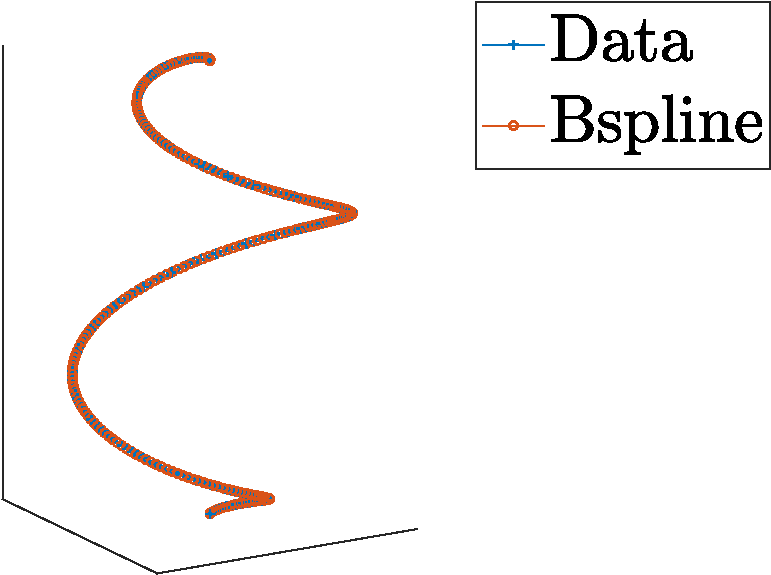
\includegraphics[width=0.42\textwidth]{snake-crop}}
&\multicolumn{2}{c||}{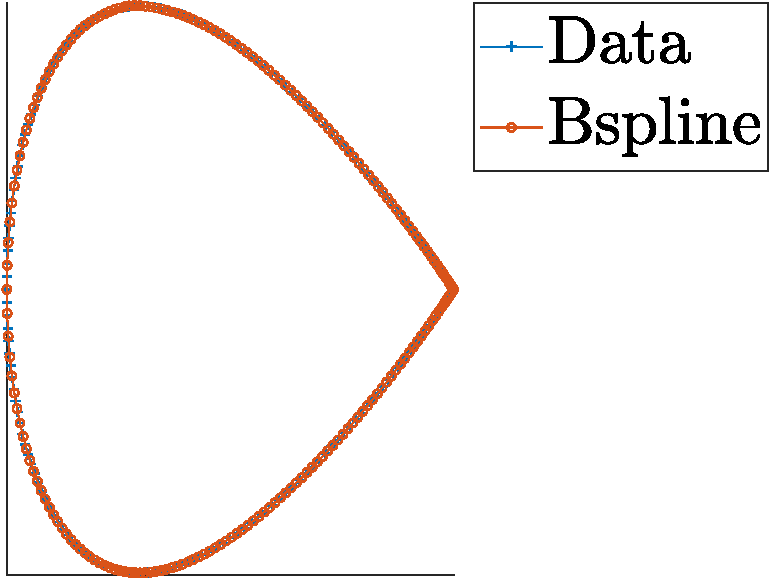
\includegraphics[width=0.42\textwidth]{naca27-crop} }\\
\hline
\end{tabular}
\caption{Results when approximating a curve moving along a sphere (see Figure \ref{fig:sphere_snake}) using 200 points.}
 \end{table}

 
 
 
 \begin{figure}
  \begin{tabular}{ccc}
  \hline
{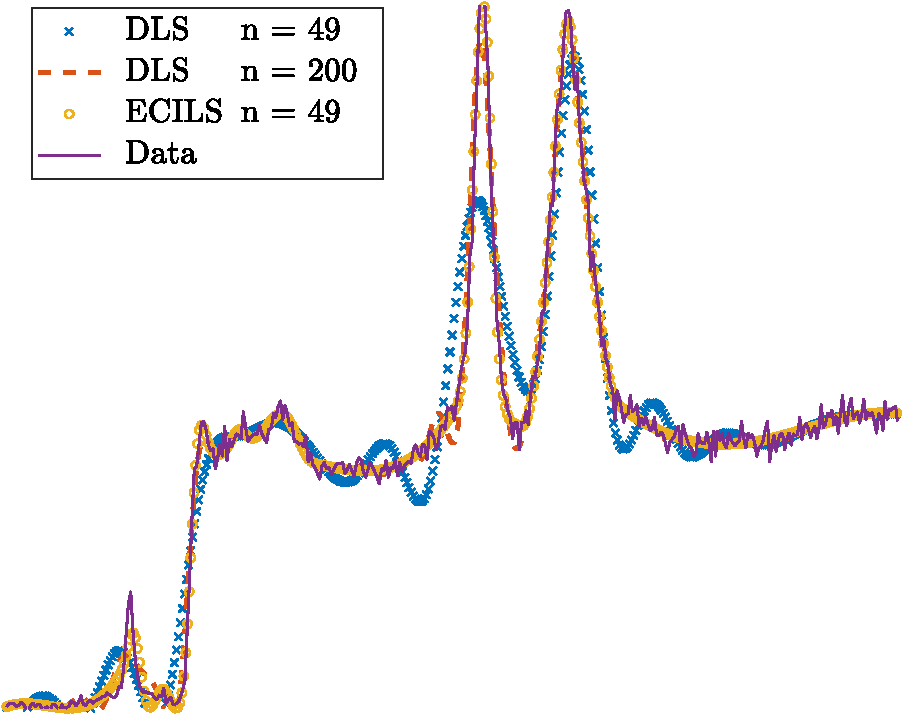
\includegraphics[width=0.29\textwidth]{noise1}}
&{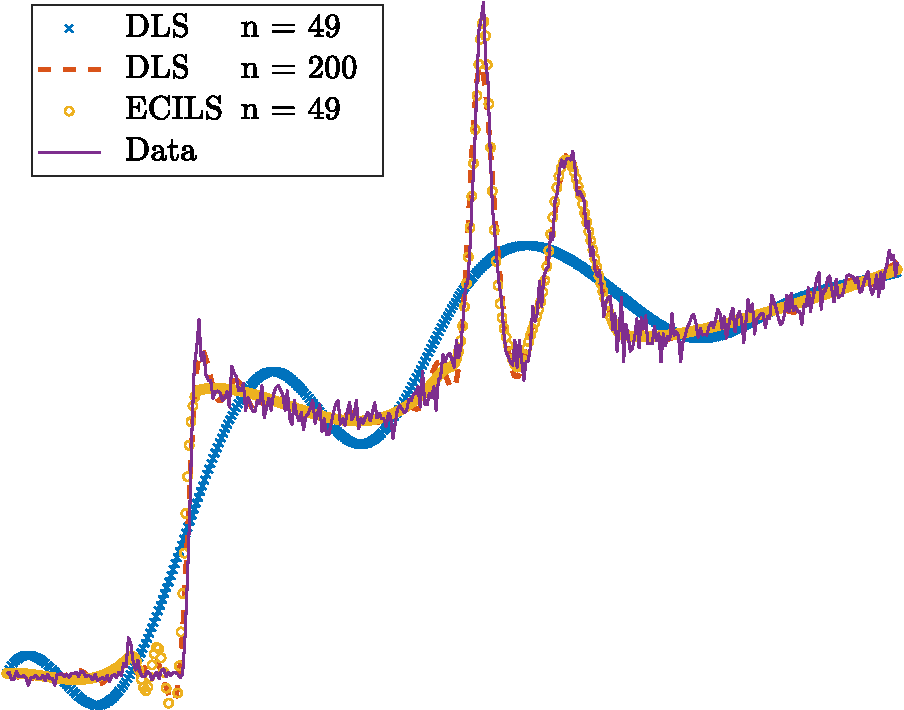
\includegraphics[width=0.29\textwidth]{noise2}}
&{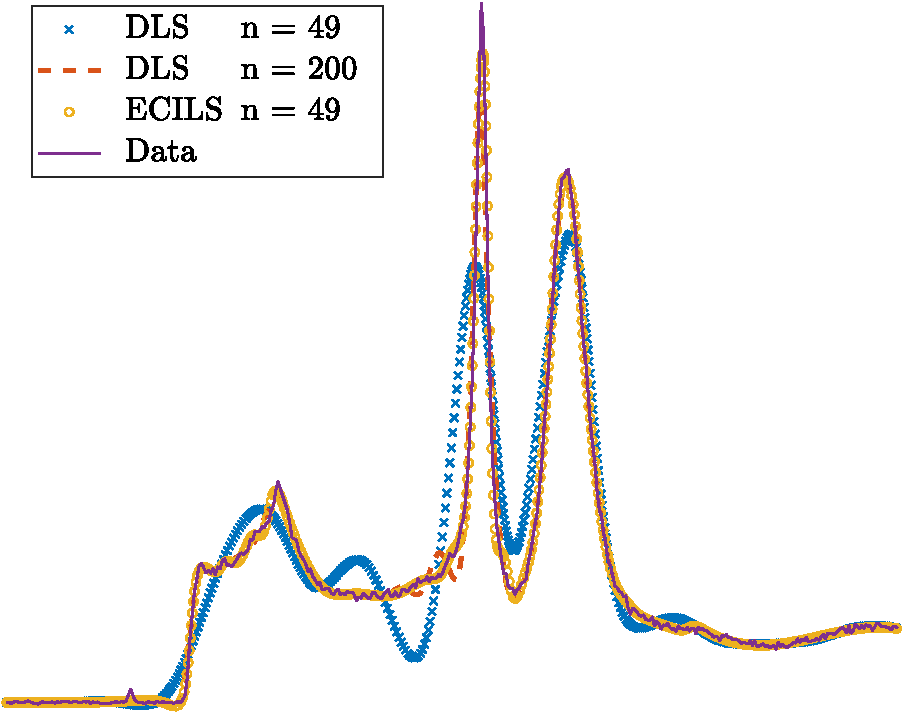
\includegraphics[width=0.29\textwidth]{noise3}}\\
\hline
  \end{tabular}
\caption{\label{fig:noise_DLS_vs_ECILS} Three data samples from Raman Spectroscopies (*) 
and the resulting approximation using the new algorithm versus a direct fit for different number of control points. 
}
 \end{figure}



 
 Figure \ref{} shows a helix obtained from \subsection{Basic Shapes Approximation}
 Consider
 
 



   




\bibliography{biblio}
 
 
 

 
 
\end{document}

 